\chapter{Model czujnika laserowego}
\label{sec:monokl}
Ponieważ czujniki laserowe tego typu są popularnie używane w robotyce, standard SDF posiada dedykowane elementy do umieszczenia takich obiektów w symulacji.
Również Gazebo posiada możliwość renderowania zasymulowanych impulsów lasera.
Tak, jak model platformy, ten pakiet otrzymał nazwę kodową \texttt{monokl}, ponieważ pozwala obserwować otoczenie, jak okular.

\section{Obliczenia symulatora}
	Czujnik laserowy jest bardzo łatwo zasymulować w przestrzeni wirtualnej za pomocą rzutowania półprostych.
	Ta technika używana jest w bardzo wielu aspektach komputerowego generowania obrazu i symulacji fizyki.

	Półprosta jest emitowana z ustalonego punktu w pewnym kierunku w przestrzeni trójwymiarowej.
	Następnie system próbuje znaleźć pierwszy punkt jej kolizji z każdym z obiektów o fizycznym kształcie, uczestniczących w symulacji.
	
	Ponieważ zasoby komputera zawsze są ograniczone, długość promienia także musi mieć pewien limit. 
	Zwykle jest on jednak na tyle duży, że z punktu widzenia obiektów uczestniczących w symulacji, w opisywanym tutaj zagadnieniu, 
	można uznać tą odległość za nieskończoną.

	Algorytm obliczania kolizji z półprostą bazuje na kosztowym porównywaniu pozycji każdego obiektu fizycznego na scenie.
	Istnieją oczywiście sposoby na zmniejszenie ilości obliczeń, na przykład metoda prostopadłościanów zawierających obiekt, ale sposób radzenia sobie z tym zagadnieniem nie jest
	częścią tematu pracy,
	Wystarczy wspomnieć, że symulacja dużej ilości laserów oraz obiektów jest operacją kosztowną.
	
	Testy pokazują, że samo ich renderowanie spowalnia symulację około czterokrotnie.
	To ze względu na bardzo dużą ich ilość, mogącą przekroczyć 1000 obliczeń kolizji w jednej klatce symulacji.

\section{Różnice między czujnikiem, a modelem}
	Półprosta emitowana jest z puntu reprezentującego środek czujnika.
	Model upraszcza rzeczywisty czujnik (budowa czujnika laserowego została opisana w sekcji \ref{sec:lidar}).
	Uproszczenie to polega na tym, iż nie ma wewnątrz zamodelowanego obiektu żadnego odpowiednika obracającego się lusterka.
	W rzeczywistym czujniku ponadto jest jeden laser, emitujący pulsy w określonych odstępach czasu.
	W modelu warto zatem emitować osobne półproste, dla każdego pulsu lasera.

	Można zauważyć tym samym, że model czujnika wydaje się funkcjonalnie lepszym, niż rzeczywisty LiDAR.
	W danej chwili, model emituje promień we wszystkich kierunkach w zakresie jednocześnie, podczas gdy czujnik jednym pulsem może dokonać tylko jednego pomiaru,
	i tylko o kącie w którym aktualnie znajduje się lusterko.
	Jednakże dyskretny sposób symulacji i sposób komunikacji urządzenia z odbiornikiem danych, powodują że w obu przypadkach dane są podawane w grupach.
	Czujnik jest wstanie wysłać pakiet z danymi z ostatniego pomiaru, podczas gdy program modelujący czujnik jest obsługiwany na zasadzie przerwań czasowych 
	po każdej klatce i tylko wtedy może wywołać funkcje zwracające dane zasymulowanych pomiarów.
	To oznacza, że interfejsy do ich obsługi zachowują się podobnie.

	Drugą rzeczą, w której model przoduje, jest nieskończona (z punktu widzenia symulacji), odległość pomiaru.
	Nie tylko jako najdalszy wykryty punkt, ale także i najbliższy. 
	Czujnik może pomijać pomiary przypadające za blisko krawędzi dozwolonego obszaru, gdyż znacznie spada w tych miejscach dokładność pomiaru, lub zwracać niedokładne dane.
	Symulator ma całkowitą dowolność w ustawianiu progu, dla którego obcina pomiar.

	Podobnie, jak w poprzednim przypadku, symulator posiada niezmienną w odległości dokładność pomiaru.
	Czujnik zmienia swoje błędy, w zależności jak daleko od niego znajduje się obiekt.

	Jednakże, w zależności od obciążenia maszyny na której uruchomiony jest symulator, model czujnika jest podatny na opóźnienia w odczytywaniu stanu.
	Fizyczny czujnik zawsze działa z tą samą częstotliwością, a jego program sterujący jest wbudowany w mikrokontroler i spełnia sztywne ramy czasowe.

\section{Komunikacja}
	Bazując na architekturze opisanej wcześniej na rysunku \ref{fig:agent}, należy tak zbudować system, aby program sterujący mógł się komunikować w identyczny sposób z 
	modelem czujnika, jak i samym czujnikiem.
	Służą do tego specjalne typy wiadomości ROSa \texttt{sensor\_msgs/LaserScan}.
	Program obsługujący model czujnika generuje i wysyła pakiety zawierające:
	\begin{itemize}
		\item Nagłówek z czasem pomiaru, identyfikatorem i ramką pozycji czujnika.
		\item Kąty początkowe i końcowe pomiaru.
		\item Odległość kątowa pomiędzy kolejnymi promieniami.
		\item Czas pomiędzy kolejnymi emisjami lasera.
		\item Czas pomiędzy tym, a poprzednim przebiegiem urządzenia.
		\item Minimalny i maksymalny dystans mierzonego obiektu od czujnika.
		\item Dane odległości.
		\item Dane jasności (jeśli czujnik posiada taką funkcjonalność).
	\end{itemize}

	Identycznie, program podłączony bezpośrednio do czujnika za pomocą jednego z interfejsów, także powinien generować takie same pakiety i udostępniać je w środowisku ROSa.

\section{Model w Gazebo}
	Tak, jak w modelu platformy, należy stworzyć odpowiedni plik SDF. 
	Warto umożliwić stosowanie modelu czujnika w modelach innych robotów. 
	Zatem jego implementacja powinna być niezależna od implementacji platformy, do której będzie przytwierdzony.
	Dodatkowo, w końcowym modelu istnieć będą dwa takie czujniki, budowa pliku powinna pozwolić na wielokrotne importowanie tych samych danych do tego samego modelu, 
	ale jednak aby były interpretowane w różny sposób (gdyż nadawcy danych muszą być rozróżnialni).

	Model składa się z dwóch elementów: korpusu i samego ,,mechanizmu'' urządzenia.
	Mechanizm przytwierdzony jest w odpowiednim miejscu korpusu, za pomocą stałego połączenia (elementu \texttt{joint}).

	Korpus posiada siatkę, reprezentującą uproszczony wygląd urządzenia, a także dwa elementy ustawiające walcowate kształty, odpowiedzialne za kolizje fizyczne.
	Teoretycznie, lepiej było by, aby model posiadał jeden walec, reprezentujący kształt urządzenia, gdyż to przyspieszyłoby symulację. 
	Jednakże, półproste emitowane ze środka obiektu, również się by z nim zderzały od wewnątrz, a co za tym idzie, nie opuszczałyby modelu czujnika.
	Element korpusu odpowiada także za przesunięcie samego lasera względem podstawy, na której całe urządzenie jest montowane, i 
	pozwala na wygodną referencję z innego modelu, w celu utworzenia wiązu.
	Jak już wcześniej wspomniano, model zawsze ma strukturę gwiazdową i więzy po stronie robota nie mogą wskazywać na element \texttt{model} czujnika, a mogą
	na obiekt korpusu.

	Główna część obiektu czujnika, skaner, posiada ozdobną siatkę, udającą czarną szybkę LiDARa, oraz element SDF \texttt{sensor}, odpowiedzialny za sam czujnik.
	W kolejnych podelementach zawierają się parametry urządzenia, takie jak ilość symulowanych laserów, ich zasięg, kąt pierwszego i ostatniego lasera, oraz współczynnik błędu pomiarowego. Ten element celowo nie ma fizycznego kształtu, aby nie blokować wychodzących półprostych. 
	Nie wpływa to na symulację, gdyż w środowisku, w którym znajduje się robot, i tak nie powinno dochodzić do kolizji modeli czujników z jakimikolwiek innymi modelami.
	Również czujniki nie są wstanie wykryć siebie nawzajem, gdyż zwrócone są do siebie martwymi kątami, a co za tym idzie nie muszą symulować nieprzezroczystych brył dla
	innych sensorów.
	W przeciwnym wypadku, element fizycznego kształtu pośrodku urządzenia byłby wymagany.

	\subsection{Połączenie modeli}
		Jak wcześniej wspomniano w sekcji \ref{sec:sdf},
		model SDF ma strukturę gwiazdową. 
		Zagnieżdżenie modeli spowodowałoby, że powstałaby inna struktura, drzewiasta.
		Dlatego też, element \texttt{import} nie umieszcza w swoim miejscu całego modelu z innego pliku, a raczej importuje jego składowe i umieszcza równolegle do istniejących.
		To oznacza, że zadbać trzeba także o więzy \texttt{joint}, łączące element podstawy platformy z podstawą czujnika, inaczej symulator uznałby łączony obiekt za dwa osobne modele.
		Potrzebna jest zatem znajomość nazw elementów składowych importowanego modelu.
		Element importowanego modelu jest tracony, pozostaje jedynie przedrostek nazwy w zaimportowanych składowych.
		Zatem program sterujący czujnikiem powinien na podstawie tylko nazwy swojego obiektu ustawić przedrostek swojego interfejsu nadawania wiadomości.

		Taka mechanika działania wydaje się mało zrozumiała i nieintuicyjna, jednak doskonale dba o zachowanie spójności modelu.
		Wszystko nadal pozostaje gwiazdą i każdy element musi być odpowiednio połączony z pozostałymi, aby dokładnie określić fizykę interakcji.
		Nie powstają niedopowiedziane sytuacje, w których zachowanie jakichś elementów byłoby nieokreślone.

		Alternatywnie, zawsze jest możliwość stworzenia dwóch, osobnych modeli czujników, tudzież całość zapisać w jednym pliku.
		Jednak takie rozwiązanie niszczy komponentową budowę środowiska i nie pozwala na użycie składowych modeli w innych modelach.
		
		\begin{figure}[h]
		\centering
		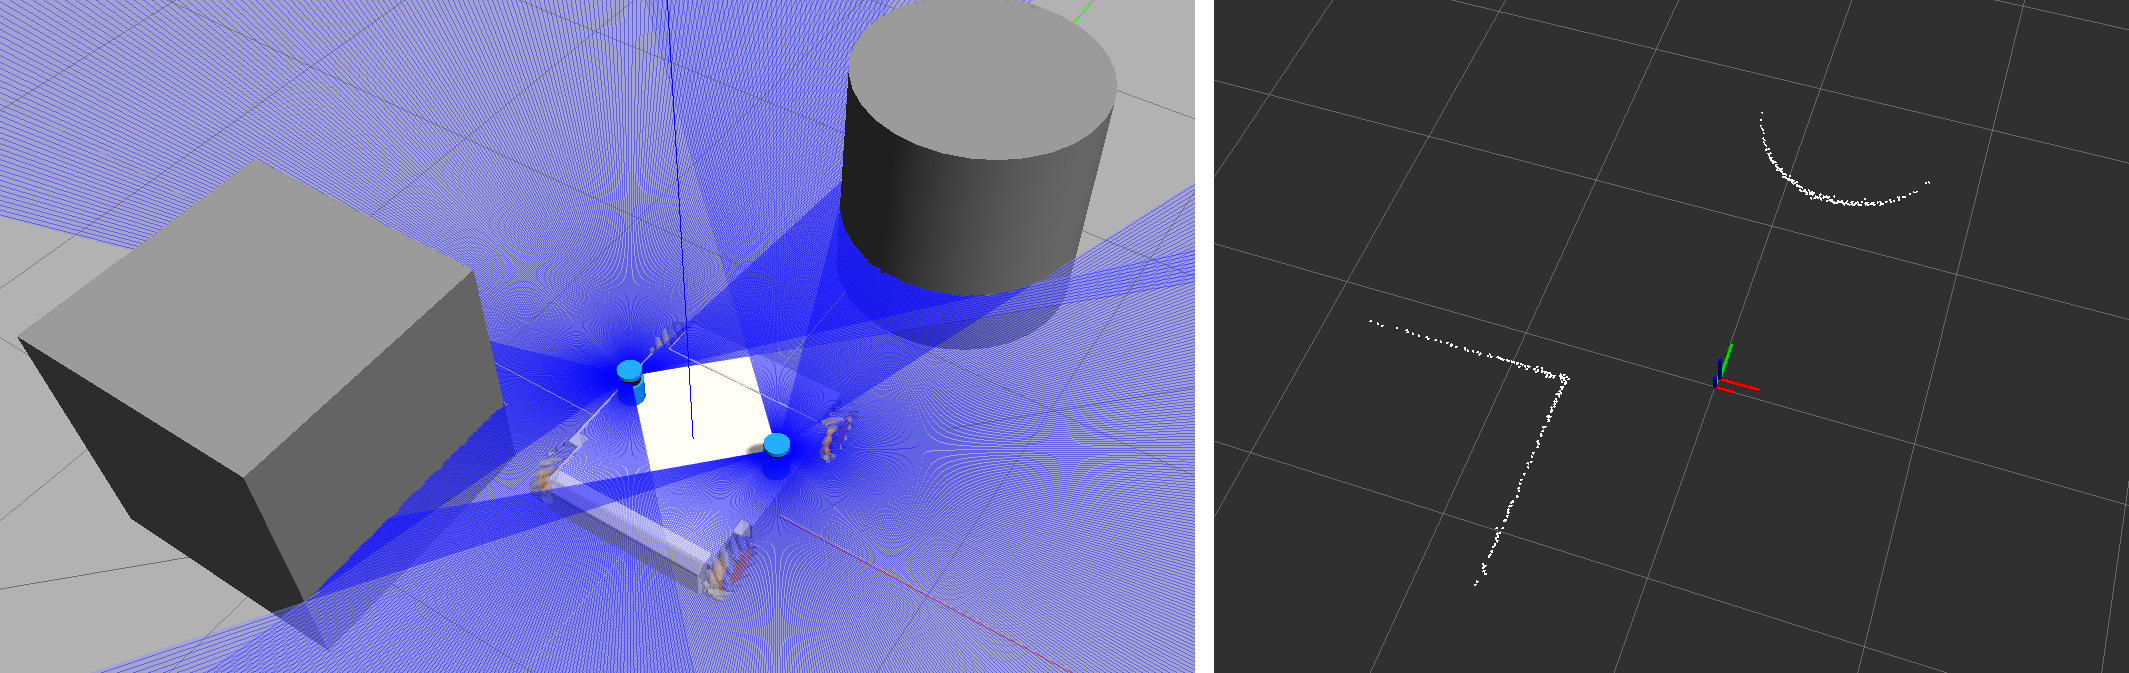
\includegraphics[width=\textwidth]{graphics/scan.png}
		\caption{Zrzut ekranu platformy z Gazebo i wygenerowane dane, obserwowane w Rviz.}
		\label{fig:scan}
		\end{figure}
		
	\subsection{Mechanika ramek}
		\label{sec:frames}
		Komunikacja poprzez pakiety wiadomości nie jest jedynym sposobem na przekazywanie informacji w środowisku ROS.
		Istnieje także mechanika ramek transformacji \texttt{TF2}.
		Jest to idea podobna do niezaimplementowanej funkcjonalności Gazebo, ale nie jest automatyczna i nie ogranicza się tylko do jednego programu.
		
		Ramka transformacji jest informacją o aktualnej pozycji i rotacji jakiegoś obiektu względem innego.
		Polega na wysłaniu pakietu typu \texttt{geometry\_msgs/TransformStamped} prosto do demona ROS.
		Pakiet zawiera:
		\begin{itemize}
			\item Nagłówek z czasem nadania ramki i identyfikatorem, oraz informacją względem jakiej ramki podane są poniższe dane.
			\item Nazwa nowej ramki, jaka powstanie po zastosowaniu podanej transformacji do określonej w nagłówku ramki.
			\item Lokalna pozycja.
			\item Lokalna rotacja.
		\end{itemize}
		Demon ROSa następnie zbiera wszystkie dane ze wszystkich nadających komponentów i oblicza hierarchę transformacji obiektów.
		Zwraca te dane na zapytania od innych komponentów.
		
		Przykładowo, gdyby symulacja robota nie odbywałaby się w przestrzeni wirtualnej, w maszynie symulacyjnej fizyki, 
		informacja o dokładnym położeniu obiektu składowego w lokalnym układzie współrzędnych wcale nie musiałaby być łatwo dostępna.
		Ma to szczególne znaczenie dla skomplikowanych mechanizmów, na przykład wielosegmentowego ramienia manipulacyjnego.
		Obliczenie pozycji i rotacji końcówki ramienia wymagałoby informacji o aktualnych pozycjach i rotacjach wszystkich segmentów.
		Która część systemu miałaby zajmować się obliczeniami i jaki kod powinien posiadać i gdzie przekazywać te informacje?
		
		Demon ROSa działa tutaj jak trzecia strona, zbierająca dane od przegubów i obliczająca pozycje i rotacje wszystkich punktów.
		W takim przypadku, każdy segment symulacji mógłby przekazywać swój identyfikator, identyfikator obiektu którym steruje, jego pozycję i rotację do demona ROSa.
		Inne programy, na przykład do wizualizacji, mogłyby wtedy zapytać się demona o dokładne pozycje przegubów w przestrzeni kartezjańskiej, a on obliczyłby je i zwrócił wynik.
		
		W symulacji platformy wielokierunkowej, mechanika ramek jest potrzebna, gdyż pakiet zwierający pomiary z czujnika laserowego nie posiada informacji o aktualnej
		pozycji samego czujnika w przestrzeni, a jedynie identyfikator ramki czujnika. 
		Pozycja potrzebna jest programowi obliczającemu pozycję z czujników i ewentualnemu wizualizatorowi samych danych.
		
		Symulator platformy zawiera drugi program, który w każdym cyklu symulacji nadaje demonowi ROS pozycje i rotacje środków czujników laserowych, dla uproszczenia
		względem początku układu współrzędnych, punktu (0,0,0). 
		Program sterujący modelem samej platformy także nadaje ramkę z pozycją i rotacją platformy względem globalnego środka układu współrzędnych.
		Dokładnie taki sam efekt byłby, gdyby nadawać stałą pozycję i rotację czujników laserowych, ale względem ramki platformy (nadawanej przez inny sterownik).
		Stałą, ponieważ czujniki nie zmieniają swojej pozycji na platformie, są przytwierdzone na stałe.
		
		\begin{table}
			\centering
			\begin{tabular}{l r}
				Punkt ramki & Nazwa punktu \\
				\hline
				Stały środek mapy & \texttt{map} \\
				Środek platformy & \texttt{omnivelma} \\
				Środek platformy kinematycznej & \texttt{pseudovelma} \\
				Emiter prawego lasera & \texttt{monokl\_r\_heart} \\
				Emiter lewego lasera & \texttt{monokl\_l\_heart} \\
			\end{tabular}
			\caption{Nazwy identyfikatorów ramek, używanych w symulatorze.}
			\label{tab:frames}
		\end{table}
			
		\begin{table}
			\centering
			\begin{tabular}{l c r}
				Nazwa & Punkt względny & Punkt danych \\
				\hline
				Pozycja i rotacja platformy & \texttt{map} & \texttt{omnivelma} \\
				Pozycja i rotacja platformy kinematycznej & \texttt{map} & \texttt{pseudovelma} \\
				Pozycja i rotacja prawego czujnika & \texttt{map} & \texttt{monokl\_r\_heart} \\
				Pozycja i rotacja lewego czujnika & \texttt{map} & \texttt{monokl\_l\_heart} \\
			\end{tabular}
			\caption{Ramki wysyłane do demona ROS.}
			\label{tab:frame_send}
		\end{table}

\section{Błędy}
	Jak podano wcześniej w tabelce \ref{tab:lidar}, wyróżnione są dwa typy błędów pomiaru, systematyczny i pomiarowy.
	Dodatkowo istnieje także błąd gruby.
	Model czujnika powinien uwzględniać wszystkie błędy, aby zwracać dane jak najbardziej zbliżone do LiDARa.

	\subsection{Błąd gruby}
		Najprostszy typ błędu polega na dużych odchyłach niektórych pomiarów od pozostałych wartości.
		W trakcie przetwarzania odczytu, te punkty powinno się odrzucić.
		Nie mniej jednak, to zadanie należy do programu sterującego, więc należy umożliwić mu testowanie tej funkcjonalności poprzez wprowadzenie takich błędów do zasymulowanych odczytów.

		Najczęstszym przypadkiem błędu grubego jest brak odbioru wysłanego impulsu. 
		To skutkuje nadaniem aktualnemu pomiarowi wartości maksymalnej, co jest bardzo łatwo wykryć i usunąć.

		Innym problemem może być odebranie światła niepochodzącego od emitera urządzenia, a jakiegoś zewnętrznego źródła.

		Ponieważ rozkład i częstotliwość tych błędów zależy od środowiska w jakim działa czujnik, bardzo ciężko jest dobrać odpowiedni algorytm ich generacji.
		%TODO dopisać po implementacji

	\subsection{Błąd systematyczny}
		Ten błąd jest stałą wartością, dodaną do każdego pomiaru.
		Spowodowany jest niedoskonałością budowy elementów pomiarowych, niewłaściwą kalibracją, zużyciem, lub otoczeniem w jakim pracuje czujnik.

		Rzeczywisty LiDAR powinien być skalibrowany przed użyciem właśnie po to, aby wewnętrzny program sterujący mógł obliczyć aktualne zboczenia pomiarów
		i skorygować dane przed wysłaniem ich wyżej.
		Czujnik może także wysyłać czyste i obarczone błędami dane do programu sterującego, który samodzielnie je skoryguje.
		Pozwoli to na zastosowanie dowolnych algorytmów oczyszczania danych, kosztem większego obciążenia programu sterującego.

		Symulator czujnika powinien mieć interfejs do ustawienia tej wartości, aby mógł być ,,skalibrowany'' w taki sam sposób, jak faktyczne urządzenie.
		%TODO dopisać po implementacji

	\subsection{Błąd pomiarowy}
		Jest to mała, losowa wartość, dodana do każdego pomiaru.
		Wynika ona z niedoskonałości samego czujnika, nieznanych zakłóceń i niezbadanych efektów kwantowych.
		Nie da się w żaden sposób usunąć, zmniejszyć, lub przewidzieć tego typu błędów.
		Jedynym sposobem jest obliczenie średniej błędu na podstawie dużej ilości pomiarów.

		Błąd pomiarowy ma zwykle rozkład normalny o określonym odchyleniu standardowym.
		Standard SDF przewiduje element określający tę liczbę, a Gazebo może wewnętrznie obliczyć i dodać do wyników odpowiednią wartość.
		Również producent podał w tabeli danych urządzenia obliczony rozkład standardowy.

		W związku z tym, wartość podana przez producenta, podana w tabelce \ref{tab:lidar}, może być bezpośrednio zapisana do 
		elementu odchylenia standardowego, w pliku SDF opisującym czujnik.
		Wadą takiego rozwiązania jest niemożność modyfikacji tego parametru w trakcie wykonywania programu, gdyż Gazebo nie wystawia API do modyfikacji tej wartości.
		Aby temu zaradzić, wystarczy obliczać błąd standardowy w programie sterującym i manualnie dodawać go do zwróconej przez symulator tablicy danych.
		Funkcje do obliczania błędu standardowego zostały wprowadzone do standardu języka C++ w 2011 roku.
		
		Na zrzucie ekranu \ref{fig:scan} można zobaczyć, iż punkty pomiarów, wizualizowane w RViz, nie leżą idealnie na figurach powstałych poprzez przecięcia skanowanych brył.
		Dodany jest szum, jak gdyby rozmazujący punkty.



